\documentclass[svgnames,smaller,10pt]{beamer}

\usetheme{metropolis}

\usepackage[utf8]{inputenc}
\usepackage[french]{babel}
\usepackage{hyperref}
\hypersetup{
    unicode=true,          
    psdextra=true,         % Aide à mieux interpréter certains symboles
    pdfencoding=auto,
}
\usepackage[T1]{fontenc}
\usepackage{geometry}
\geometry{
    left=2.5mm,
    right=2.5mm,
    top=0mm,
    bottom=0mm
}
\usepackage{amssymb} % pour \blackdiamond
\usepackage{tikz}
\usepackage{graphicx,animate}
\usepackage{media9}
\usepackage{subcaption}


\newcommand{\replacementchar}{%
  \tikz[baseline=-0.6ex]{
    %\node[inner sep=0pt] (d) {\Large$\blackdiamond$};
    \node[inner sep=0pt] (d) {\Large$\blacksquare$};
    \node[white, font=\scriptsize\bfseries] at (d.center) {?};
  }%
}
\usepackage{tabularx}
%\usepackage[style=alphabetic,citestyle=authoryear]{biblatex}
%\addbibresource{bibliographie.bib}

\usepackage{xspace}
\newcommand{\themename}{\textbf{\textsc{metropolis}}\xspace}
\title{L2S4: Édition numérique\\
TD 9: Les écritures profilaires : quelles contraintes éditoriales?
}

\date{}
\author{Marine Tiger\\   \texttt{marine.tiger@sorbonne-universite.fr}}

\institute{Littératures françaises et comparée ED19, CELLF, Sorbonne Université}

\begin{document}
\maketitle
\setbeamertemplate{section in toc}[sections numbered]

\section{Atelier: créer un profil et publier}
\begin{frame}{Atelier: créer un profil et publier}
    \centering
    
\includegraphics[width=.4\textwidth]{Images/qrcode_atelier.png}
\end{frame}
\section{Introduction}
\begin{frame}{Rappel: le profil, une écriture de soi}
    L'écriture profilaire = mise en scène de soi.\\
    \vspace{1em}
    Permet la réappropriation de la fonction auctoriale par les artistes.
\end{frame}
\begin{frame}{Les contraintes éditoriales des plateformes}
    Rappel que la plateforme n'est pas un support neutre:
    \begin{itemize}
        \item \textbf{Le symbole de l'autorité} (certification, nombre d'abonnés)
        \item \textbf{La standardisation du style} (usage des hashtags, limite de caractères etc...)
        \item \textbf{Une éditorialisation "invisible"} (algorithme de recommandation)
    \end{itemize}
\end{frame}





\begin{frame}{Problématique}
    Que disent ces contraintes sur les politiques d'éditorialisation? Quels enjeux pour les utilisateur.rices? 
\end{frame}

\section{Architexte et computexte}
\begin{frame}{Définitions}
    Deux notions développées par Alexandra Saemmer, dans \href{https://shs.cairn.info/revue-communication-et-langages-2020-1-page-99?lang=fr}{\textit{De l’architexte au computexte Poétiques du texte numérique, face à l’évolution des dispositifs}}, 2020:\\
    \begin{itemize}
        \item \textbf{Architexte:} les cases à cocher, les formulaires à remplir, les polices de caractères, couleurs prédéfinies etc...\\
        \textrightarrow{} Contraintes visibles.
        \item \textbf{Computexte:} les contraintes de contenu.
    \end{itemize}
\end{frame}

\begin{frame}{Définitions}
    \begin{block}{}
    On écrit plus dans ces outils mais avec eux. Voire ils écrivent même à notre place.\\
    \textbf{Exemple:} l'auto-complétion.
    \end{block}
    \begin{block}{}
        Rappel exemple des générateurs de texte: l'objectif était de compléter des phrases en appliquant les règles linguistiques.\\
        \textrightarrow{} Les plateformes complètent avec des algorithmes.
    \end{block}
\end{frame}

\begin{frame}{Des dispositifs d'écriture}
    \begin{itemize}
        \item Le nombre de caractères
        \item Le cadre carré d'Instagram
        \item Les émojis sur Facebook
    \end{itemize}
\end{frame}

\begin{frame}{Exemple: la Broetry sur LinkedIn}
    \begin{columns}
    % Colonne de gauche : Texte
        \begin{column}{0.4\textwidth}
            \begin{itemize}
                \item Billet de blog de Carina Rampelt (\url{https://fenwick.media/rewild/magazine/dead-broets-society-behind-the-strange-story})
                \item Forme de storytelling sur LinkedIn
                \item Pousser les gens à cliquer sur "voir plus", ce qui signale à LinkedIn que vous êtes intéressées
            \end{itemize}
        \end{column}

        % Colonne de droite : Image
        \begin{column}{0.5\textwidth}
            
\includegraphics[width=.9\columnwidth]{Images/Broetry.png}
            
        \end{column}
    \end{columns}
\end{frame}

\begin{frame}{Exemple: la Broetry sur LinkedIn}
    Carina Rampelt décrit les règles de la Broetry comme suit:
    \begin{itemize}
        \item Une phrase d'ouverture "\textit{click bait}"
        \item Le contenu: une anecdote personnelle
        \item Le format: court, phrase simple avec des sauts de ligne 
        \item La phrase de conclusion: une leçon de vie cliché ou "\textit{inspirational quote}"
    \end{itemize}
\end{frame}

\begin{frame}{Exemple: la Broetry sur LinkedIn}
    \centering
    
\includegraphics[width=.6\textwidth]{Images/broetry_regles.png}
\end{frame}

\section{Optimiser ses publications}
\begin{frame}{Exemple: la série Été d'Arte sur Instagram}
    \begin{columns}
    % Colonne de gauche : Texte
        \begin{column}{0.4\textwidth}
            \begin{itemize}
                \item Exemple présenté par \href{https://art-et-reseaux.fr/ete-social-graphic-novel-sur-instagram/}{Nolwenn Tréhondart}
                \item  BD publiée sur Instagram avec la boîte \textit{Bigger than fiction}
                \item Idée est d'introduire de l'art, de la fiction, de la culture et du politique.\\
                \textrightarrow{} Comment capter les utilisateur.rices en respectant les contraintes de la plateforme? 
            \end{itemize}
        \end{column}

        % Colonne de droite : Image
        \begin{column}{0.5\textwidth}
            
\includegraphics[width=.9\columnwidth]{Images/profil_ete_arte.png}
            
        \end{column}
    \end{columns}
\end{frame}

\begin{frame}{Exemple: la série Été d'Arte sur Instagram}
    \begin{center}
         {\small \textit{ "Les technologies qui permettent d’écouler les marchandises se sont déplacées en une quinzaine d’années du produit au logo, puis du logo aux stories."}}\\
    \textbf{Christian Salmon, \textit{Storytelling, la machine à fabriquer des histoires et à formater les esprits}}
    \end{center}
   
    On cherche des histoires auxquelles on peut s'identifier (\textit{"relatable"}).

\end{frame}

\begin{frame}{Exemple: la série Été d'Arte sur Instagram}
    \begin{itemize}
        \item Chaque épisode doivent se comprendre indépendament des autres.
        \item Respecter la limite de 10 cases par post (au moment de la publication)
        \item Les hashtags sont utilisés comme légende
        \item Mélange de musique, animation et images.
    \end{itemize}
\end{frame}


\begin{frame}{Exemple: la série Été d'Arte sur Instagram}
    \begin{center}
        Cas intéressant: s'adapter à un changement d'algorithme.
    \end{center}
\vspace{1em}
\begin{columns}
    % Colonne de gauche : Texte
        \begin{column}{0.5\textwidth}
            \centering
            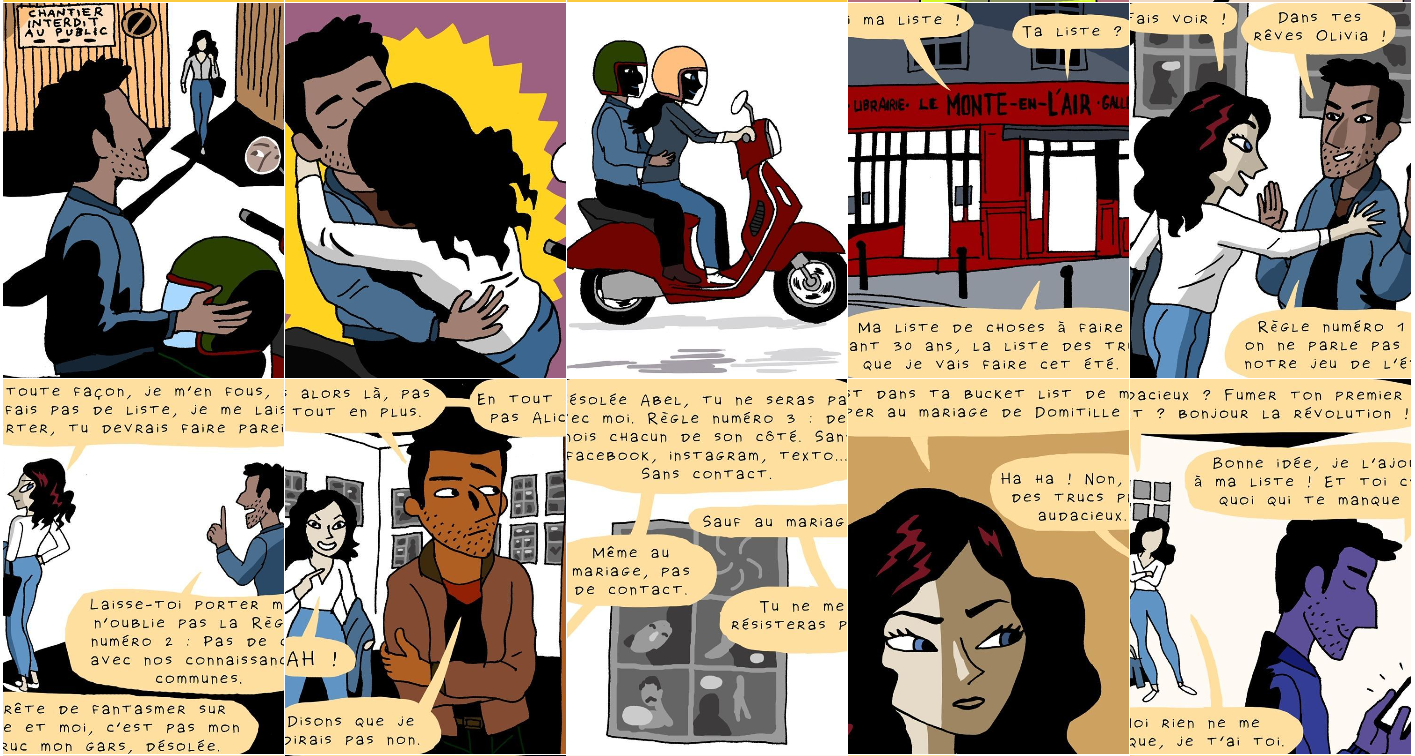
\includegraphics[width=.9\columnwidth]{Images/ete_arte_ancien.png}
            
        \end{column}

        % Colonne de droite : Image
        \begin{column}{0.5\textwidth}
            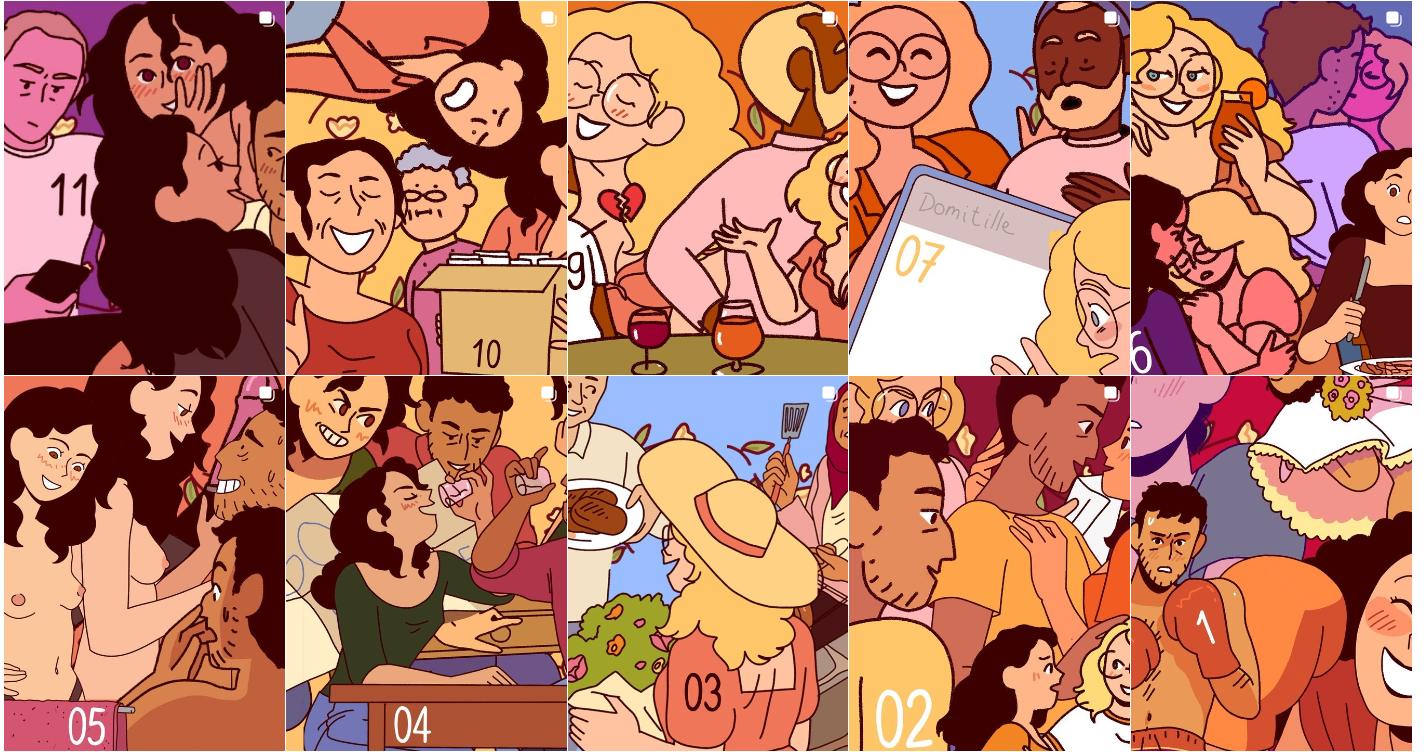
\includegraphics[width=.9\columnwidth]{Images/ete_arte_recent.png}
            
        \end{column}
    \end{columns}

\end{frame}



\section{Les contraintes normatives et algorithmiques: exemple du \textit{shadow banning}}
\begin{frame}{Définitions}
    Deux types de modération:
    \begin{itemize}
        \item La suppression de contenus
        \item L'invisibilisation (\textit{shadow ban})
    \end{itemize}

    Définition de Caroline Are: "\textit{a form of light censorship targeting “vaguely inappropriate content” that is hidden from the platform’s explore page"}\\
\vspace{1em}
    Définition de Thibault Grison: \textit{"Pour ma part, je parle de déréférencement comme stratégie de modération silencieuse."}
\end{frame}

\begin{frame}{L'invisibilisation de contenu}
    \begin{center}
       {\small \textit{"[...] l’éditorialisation des contenus dans les RSN s’apparente en fait à une hiérarchisation de ce
qui est rendu plus ou moins invisible auprès de l’ensemble ou d’une partie des publics."}}\\
\textbf{Thibault Grison, \textit{Faire dire, faire taire : la modération (algorithmique) des réseaux sociaux numériques au prisme des sexualités}, 2024}
    \end{center}
\end{frame}

\begin{frame}{L'invisibilisation de contenu}
    \begin{itemize}
        \item Le blocage géographique;
        \item Le déréférencement automatique via les hashtags;
        \item La démonétisation;
        \item L'altération des modalités de consultations
    \end{itemize}
\end{frame}

\begin{frame}{Exemple d'intervention d'État}
    \centering
    
\includegraphics[width=.6\textwidth]{Images/indonesie_blocage.png}
    
\end{frame}

\begin{frame}{Exemple: l'\textit{origine du monde} et la censure de Facebook}
    \begin{columns}
    % Colonne de gauche : Texte
        \begin{column}{0.5\textwidth}
            \centering
            
\includegraphics[width=.9\columnwidth]{Images/lemonde_origine_monde.png}
            
        \end{column}

        % Colonne de droite : Image
        \begin{column}{0.5\textwidth}
            
\includegraphics[width=.9\columnwidth]{Images/article_origine_monde.png}
            
        \end{column}
    \end{columns}
\end{frame}

\begin{frame}{Déférencement d'hastag: exemple de l'anorexie sur TikTok}
    \begin{columns}
    % Colonne de gauche : Texte
        \begin{column}{0.5\textwidth}
            \centering
            
\includegraphics[width=.6\columnwidth]{Images/anorexie_tiktok.png}
            
        \end{column}

        % Colonne de droite : Image
        \begin{column}{0.5\textwidth}
            \centering
            
\includegraphics[width=.6\columnwidth]{Images/TCA_tiktok.png}
            
        \end{column}
    \end{columns}
\end{frame}

\begin{frame}{Mais aussi la modération de profil}
    \begin{itemize}
        \item Bannissement temporaire d'un compte 
        \item \textit{Shadow banned}
    \end{itemize}
\end{frame}

\begin{frame}{Une modération invisible?}
    Prise de parole à ce sujet de la tiktokeuse Grandebavardeuse
\end{frame}

\begin{frame}{Les chartes de modération}
    % La modération fait partie du travail d'éditorialisation des réseaux sociaux = les comptes et posts ne sont pas juste supprimés.\\
    \textbf{\textit{Terms of service}}: des sortes de contrat de consommation entre l'internaute et la plateforme.\\
    \vspace{1em}
    // \\
    \vspace{1em}
    \textbf{Les chartes de modération}: "\textit{[...] des instructions données aux utilisateur·rice·s – qui, pour la majeure partie d’entre eux et elles ne les liront jamais – et comme des textes – dont l’existence même agit comme une performance discursive ’auto-légitimation
de l’entreprise à supprimer, recommander ou invisibiliser un contenu ou un profil}" (Thibault Grison)
\end{frame}

\begin{frame}{Les chartes de modération}
    Les règles définies leur sont spécifiques et en même temps elles sont interdépendantes entre les plateformes:
    \begin{itemize}
        \item Meta est le groupe de Facebook et Instagram;
        \item Meta a ses applications sur l'\textit{Apple Store} qui a ses propres règles.
    \end{itemize}
\end{frame}

\begin{frame}{Les chartes de modération}
    \begin{center}
        {\small \textit{Il faut donc bien comprendre que les règles communautaires des RSN sont dépendantes de tout un écosystème d’acteurs : l’entreprise–mère (Meta, par exemple), les entreprises détentrices des systèmes d’exploitation (Apple, par exemple) mais aussi des autorités publiques– qui instaurent des cadres juridiques contraignants en matière de liberté d’expression – selon les pays dans lesquels les entreprises opèrent.}}\\
        \textbf{Thibault Grison, \textit{Faire dire, faire taire : la modération (algorithmique) des réseaux sociaux numériques au prisme des sexualités}, 2024}
    \end{center}
\end{frame}

\begin{frame}{Pour résumer}
    \begin{columns}
    % Colonne de gauche : Texte
        \begin{column}{0.5\textwidth}
            \textbf{La modération visible}
            \centering
            \begin{itemize}
                \item Post supprimé avec notification
                \item Compte suspendu ou banni
                \item Procédure de recours possible
                \item Règles documentées dans les CGU
            \end{itemize}
        \end{column}

        % Colonne de droite : Image
        \begin{column}{0.5\textwidth}
            \textbf{Le \textit{shadowbanning}}
            \centering
            \begin{itemize}
                \item Le post reste en ligne mais n'est plus diffusé
                \item Aucune notification 
                \item Critères opaques, non publiés officiellement
            \end{itemize}
            
        \end{column}
    \end{columns}
\end{frame}

\begin{frame}{Des expériences pour pousser les limites des algorithmes}
    Dans \textit{De l’architexte au computexte Poétiques du texte numérique, face à l’évolution des dispositifs.}, Alexandra Saemmer présente deux exemples:
    \begin{itemize}
        \item Jean-Pierre Balpe : maintient une vingtaine de comptes Facebook pour observer et tester les mécanismes algorithmiques de la plateforme.
        \item Rachel Charlus : plasticienne qui publie des sculptures et peintures représentant des corps dénudés, testant les limites de la modération du nu artistique.
    \end{itemize}
\end{frame}


\section{Contourner les règles: \textit{algospeak} et crypto-langages}
\begin{frame}{\textit{Algospeak}}
\textbf{Algospeak} = ensemble des stratégies linguistiques développées pour contourner la modération algorithmique.\\
\textbf{Principe} : remplacer les termes sensibles par des codes, euphémismes, néologismes, émojis. \\
Théorisé par Adam Aleksic, linguiste américain.
\end{frame}

\begin{frame}{Crypto-langages}
    Expression théorisée par Alexandra Saemmer dans \textit{Le parler fransais des Gilles et John. Enquête sur les crypto-langages militants au sein des plateformes} (2019.)\\
    Ce sont des codes collectifs, un langage parallèle lisible par leur communauté.\\
    Exemple: les gilets jaunes.\\
    \vspace{1em}
    Problème: sert aussi à dissimuler des discours dangereux
\end{frame}

\begin{frame}{Crypto-langages}
    Quelques exemples qu'on peut trouver dans l'article d'A. Saemmer:
    \begin{itemize}
        \item macrotte (Macron)
        \item blinder (blindés)
        \item Cast’amere
        \item Gilles et John
    \end{itemize}
\end{frame}

\section{Conclusion}
\begin{frame}{Conclusion}
    \begin{itemize}
        \item Les plateformes ne sont pas de simples supports: éditorialisation active qui façonnent les textes, les identités et les récits.
        \item L'écriture profilaire est toujours une négociation entre intention de l'auteur·rice, contraintes formelles, logiques algorithmiques et normes communautaires.
        \item Les pratiques de résistance (algospeak, crypto-langages, comptes multiples) montrent que les usager·es ne sont pas passif·ves

    \end{itemize}
  
\end{frame}
\end{document}